\documentclass[]{article}
\usepackage{lmodern}
\usepackage{amssymb,amsmath}
\usepackage{ifxetex,ifluatex}
\usepackage{fixltx2e} % provides \textsubscript
\ifnum 0\ifxetex 1\fi\ifluatex 1\fi=0 % if pdftex
  \usepackage[T1]{fontenc}
  \usepackage[utf8]{inputenc}
\else % if luatex or xelatex
  \ifxetex
    \usepackage{mathspec}
  \else
    \usepackage{fontspec}
  \fi
  \defaultfontfeatures{Ligatures=TeX,Scale=MatchLowercase}
  \newcommand{\euro}{€}
\fi
% use upquote if available, for straight quotes in verbatim environments
\IfFileExists{upquote.sty}{\usepackage{upquote}}{}
% use microtype if available
\IfFileExists{microtype.sty}{%
\usepackage{microtype}
\UseMicrotypeSet[protrusion]{basicmath} % disable protrusion for tt fonts
}{}
\usepackage[margin=1in]{geometry}
\usepackage{hyperref}
\PassOptionsToPackage{usenames,dvipsnames}{color} % color is loaded by hyperref
\hypersetup{unicode=true,
            pdftitle={Analysis of the Effect of Vitamin C on Tooth Growth in Guinea Pigs},
            pdfauthor={Chris Shaw},
            pdfborder={0 0 0},
            breaklinks=true}
\urlstyle{same}  % don't use monospace font for urls
\usepackage{color}
\usepackage{fancyvrb}
\newcommand{\VerbBar}{|}
\newcommand{\VERB}{\Verb[commandchars=\\\{\}]}
\DefineVerbatimEnvironment{Highlighting}{Verbatim}{commandchars=\\\{\}}
% Add ',fontsize=\small' for more characters per line
\usepackage{framed}
\definecolor{shadecolor}{RGB}{248,248,248}
\newenvironment{Shaded}{\begin{snugshade}}{\end{snugshade}}
\newcommand{\KeywordTok}[1]{\textcolor[rgb]{0.13,0.29,0.53}{\textbf{{#1}}}}
\newcommand{\DataTypeTok}[1]{\textcolor[rgb]{0.13,0.29,0.53}{{#1}}}
\newcommand{\DecValTok}[1]{\textcolor[rgb]{0.00,0.00,0.81}{{#1}}}
\newcommand{\BaseNTok}[1]{\textcolor[rgb]{0.00,0.00,0.81}{{#1}}}
\newcommand{\FloatTok}[1]{\textcolor[rgb]{0.00,0.00,0.81}{{#1}}}
\newcommand{\ConstantTok}[1]{\textcolor[rgb]{0.00,0.00,0.00}{{#1}}}
\newcommand{\CharTok}[1]{\textcolor[rgb]{0.31,0.60,0.02}{{#1}}}
\newcommand{\SpecialCharTok}[1]{\textcolor[rgb]{0.00,0.00,0.00}{{#1}}}
\newcommand{\StringTok}[1]{\textcolor[rgb]{0.31,0.60,0.02}{{#1}}}
\newcommand{\VerbatimStringTok}[1]{\textcolor[rgb]{0.31,0.60,0.02}{{#1}}}
\newcommand{\SpecialStringTok}[1]{\textcolor[rgb]{0.31,0.60,0.02}{{#1}}}
\newcommand{\ImportTok}[1]{{#1}}
\newcommand{\CommentTok}[1]{\textcolor[rgb]{0.56,0.35,0.01}{\textit{{#1}}}}
\newcommand{\DocumentationTok}[1]{\textcolor[rgb]{0.56,0.35,0.01}{\textbf{\textit{{#1}}}}}
\newcommand{\AnnotationTok}[1]{\textcolor[rgb]{0.56,0.35,0.01}{\textbf{\textit{{#1}}}}}
\newcommand{\CommentVarTok}[1]{\textcolor[rgb]{0.56,0.35,0.01}{\textbf{\textit{{#1}}}}}
\newcommand{\OtherTok}[1]{\textcolor[rgb]{0.56,0.35,0.01}{{#1}}}
\newcommand{\FunctionTok}[1]{\textcolor[rgb]{0.00,0.00,0.00}{{#1}}}
\newcommand{\VariableTok}[1]{\textcolor[rgb]{0.00,0.00,0.00}{{#1}}}
\newcommand{\ControlFlowTok}[1]{\textcolor[rgb]{0.13,0.29,0.53}{\textbf{{#1}}}}
\newcommand{\OperatorTok}[1]{\textcolor[rgb]{0.81,0.36,0.00}{\textbf{{#1}}}}
\newcommand{\BuiltInTok}[1]{{#1}}
\newcommand{\ExtensionTok}[1]{{#1}}
\newcommand{\PreprocessorTok}[1]{\textcolor[rgb]{0.56,0.35,0.01}{\textit{{#1}}}}
\newcommand{\AttributeTok}[1]{\textcolor[rgb]{0.77,0.63,0.00}{{#1}}}
\newcommand{\RegionMarkerTok}[1]{{#1}}
\newcommand{\InformationTok}[1]{\textcolor[rgb]{0.56,0.35,0.01}{\textbf{\textit{{#1}}}}}
\newcommand{\WarningTok}[1]{\textcolor[rgb]{0.56,0.35,0.01}{\textbf{\textit{{#1}}}}}
\newcommand{\AlertTok}[1]{\textcolor[rgb]{0.94,0.16,0.16}{{#1}}}
\newcommand{\ErrorTok}[1]{\textcolor[rgb]{0.64,0.00,0.00}{\textbf{{#1}}}}
\newcommand{\NormalTok}[1]{{#1}}
\usepackage{longtable,booktabs}
\usepackage{graphicx,grffile}
\makeatletter
\def\maxwidth{\ifdim\Gin@nat@width>\linewidth\linewidth\else\Gin@nat@width\fi}
\def\maxheight{\ifdim\Gin@nat@height>\textheight\textheight\else\Gin@nat@height\fi}
\makeatother
% Scale images if necessary, so that they will not overflow the page
% margins by default, and it is still possible to overwrite the defaults
% using explicit options in \includegraphics[width, height, ...]{}
\setkeys{Gin}{width=\maxwidth,height=\maxheight,keepaspectratio}
\setlength{\parindent}{0pt}
\setlength{\parskip}{6pt plus 2pt minus 1pt}
\setlength{\emergencystretch}{3em}  % prevent overfull lines
\providecommand{\tightlist}{%
  \setlength{\itemsep}{0pt}\setlength{\parskip}{0pt}}
\setcounter{secnumdepth}{0}

%%% Use protect on footnotes to avoid problems with footnotes in titles
\let\rmarkdownfootnote\footnote%
\def\footnote{\protect\rmarkdownfootnote}

%%% Change title format to be more compact
\usepackage{titling}

% Create subtitle command for use in maketitle
\newcommand{\subtitle}[1]{
  \posttitle{
    \begin{center}\large#1\end{center}
    }
}

\setlength{\droptitle}{-2em}
  \title{Analysis of the Effect of Vitamin C on Tooth Growth in Guinea Pigs}
  \pretitle{\vspace{\droptitle}\centering\huge}
  \posttitle{\par}
  \author{Chris Shaw}
  \preauthor{\centering\large\emph}
  \postauthor{\par}
  \predate{\centering\large\emph}
  \postdate{\par}
  \date{23 April 2016}



% Redefines (sub)paragraphs to behave more like sections
\ifx\paragraph\undefined\else
\let\oldparagraph\paragraph
\renewcommand{\paragraph}[1]{\oldparagraph{#1}\mbox{}}
\fi
\ifx\subparagraph\undefined\else
\let\oldsubparagraph\subparagraph
\renewcommand{\subparagraph}[1]{\oldsubparagraph{#1}\mbox{}}
\fi

\begin{document}
\maketitle

\section{Synopsis}\label{synopsis}

This paper analyses how dosage levels and delivery method of vitmain C
effect the length of odontoblasts (cells responsible for tooth growth)
in 60 guinea pigs. Each animal received one of three dose levels of
vitamin C (0.5, 1, and 2 mg/day) by one of two delivery methods, (orange
juice or ascorbic acid (a form of vitamin C and coded as VC).

We conclude that dose levels make a significant impact to the mean tooth
length, whereas the delivery methods do not.

\section{Exploratory Analysis}\label{exploratory-analysis}

The following table summarises the dataset. The mean and standard
deviation of cell length is show for each dosage level and each delivery
method. The number of observations in each grouping is also shown.

\begin{longtable}[c]{@{}ccccc@{}}
\caption{Summary of tooth length by supplement and
dosage}\tabularnewline
\toprule
Supplement & Dose & Num obs & Mean & Std dev\tabularnewline
\midrule
\endfirsthead
\toprule
Supplement & Dose & Num obs & Mean & Std dev\tabularnewline
\midrule
\endhead
OJ & 0.5 & 10 & 13.23 & 4.46\tabularnewline
OJ & 1.0 & 10 & 22.70 & 3.91\tabularnewline
OJ & 2.0 & 10 & 26.06 & 2.66\tabularnewline
VC & 0.5 & 10 & 7.98 & 2.75\tabularnewline
VC & 1.0 & 10 & 16.77 & 2.52\tabularnewline
VC & 2.0 & 10 & 26.14 & 4.80\tabularnewline
\bottomrule
\end{longtable}

\section{Assumptions}\label{assumptions}

The population of odontoblast cell lengths is assumed to be normally
distributed with mean \(\mu\) and variance \(\sigma^2\). The table above
ahows that the mean is very different depending on the dose and delivery
method of vitmain C.

The plots overleaf show how the length varies depending on these
variables.

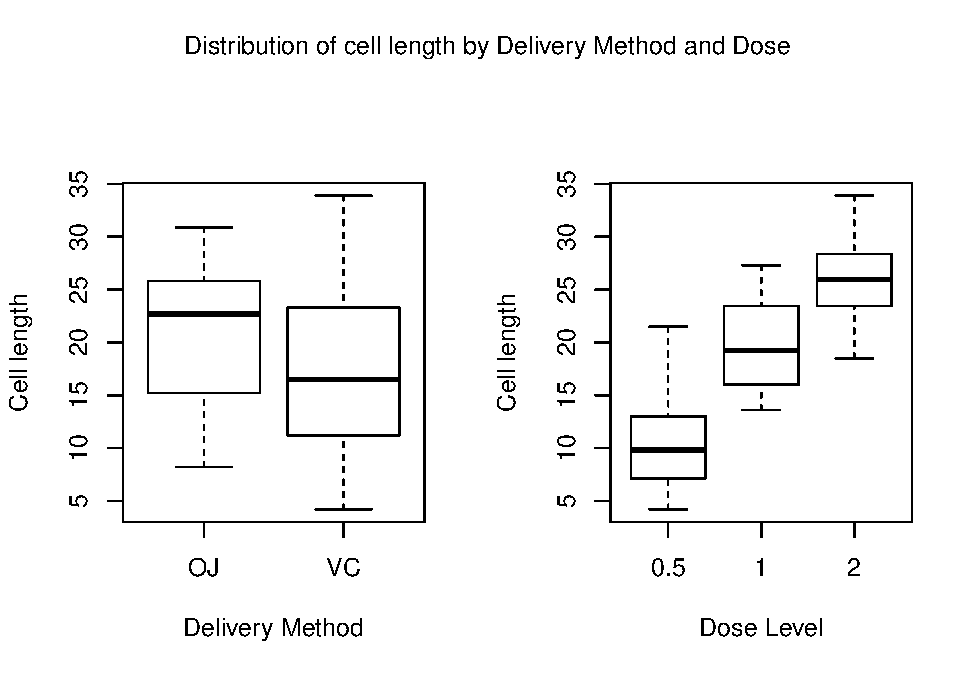
\includegraphics{wk4project-inference_files/figure-latex/boxplots-1.pdf}

Although the OJ delivery method seems to have a larger mean, the
variance of the VC method is much wider. However, when it comes to dose
levels, the mean seems to clearly increase as doseage increases.

Both of these will be examined more rigorously by hypothesis testing.

\section{Hypothesis testing}\label{hypothesis-testing}

First we compare the different supplements, OJ and VC. The mean tooth
length from the population using each of these is \(\mu_{oj}\) and
\(\mu_{vc}\) respectively. The null hypothesis, \(H_0\) is that these
means are equal, i.e: \[H_0 : \mu_{oj} = \mu_{vc}\]
\[H_a : \mu_{oj} \neq \mu_{vc}\] We want to find evidence of whether the
alternative hypothesis \(H_a\) may be true, that the means are not
equal.

A two sided t-test was performed to test this (see appendix for
details). The p-value is calculated at 0.0604. This is quite high, so we
fail to reject the null hypthosis and conclude there is no evidence that
the means are different.

\newpage

Next we compare the differences in cell length depending on dosage
level. The mean tooth length from the population for each is \(\mu_2\),
\(\mu_1\) and \(\mu_{0.5}\) respectively. The null hypothesis, \(H_0\)
is that these means are equal, i.e: \[H_0 : \mu_2 = \mu_1\]
\[H_a : \mu_2 > \mu_1\] We want to find evidence of whether the
alternative hypothesis \(H_a\) may be true, that \(\mu_2\) is greater
than \(\mu_1\).

We run a one sided t-test (see appendix) and the p-value is calculated
at 9.0541427× 10\textsuperscript{-6}. This is very low, so we reject the
null hypthosis and conclude the alternate hypothesis \(H_a\) is true.

\section{Conclusion}\label{conclusion}

The analysis of the data and the hypothesis testing leads us to the
following conclusions:

\begin{itemize}
\tightlist
\item
  It is not possible to determine whether the delivery method of orange
  juice or ascorbic acid produces a higher mean cell length.
\item
  The doseage levels however do produce a significant difference and
  enables us to say that higher doses will lead to a higher mean cell
  length.
\end{itemize}

\clearpage
\appendix
\pagenumbering{roman}

\section{Appendix}\label{appendix}

This is the code used to generate the summary table:

\begin{Shaded}
\begin{Highlighting}[]
\KeywordTok{data}\NormalTok{(ToothGrowth)}
\CommentTok{#extract measurements for each of the supplement types and dosage levels}
\NormalTok{vc<-ToothGrowth[ToothGrowth$supp==}\StringTok{"VC"}\NormalTok{,]$len}
\NormalTok{oj<-ToothGrowth[ToothGrowth$supp==}\StringTok{"OJ"}\NormalTok{,]$len}
\NormalTok{d_05<-ToothGrowth[ToothGrowth$dose==}\FloatTok{0.5}\NormalTok{,]$len}
\NormalTok{d_1<-ToothGrowth[ToothGrowth$dose==}\DecValTok{1}\NormalTok{,]$len}
\NormalTok{d_2<-ToothGrowth[ToothGrowth$dose==}\DecValTok{2}\NormalTok{,]$len}

\CommentTok{# Calculate aggregrated statistics on supp and dose (number of obs, mean and sd)}
\NormalTok{ag<-}\KeywordTok{aggregate}\NormalTok{(len~supp+dose, ToothGrowth, }
              \NormalTok{function(x) }\KeywordTok{c}\NormalTok{(}\DataTypeTok{n=}\KeywordTok{as.integer}\NormalTok{(}\KeywordTok{length}\NormalTok{(x)), }
                            \DataTypeTok{mn=}\KeywordTok{round}\NormalTok{(}\KeywordTok{mean}\NormalTok{(x),}\DecValTok{2}\NormalTok{), }
                            \DataTypeTok{sd=}\KeywordTok{round}\NormalTok{(}\KeywordTok{sd}\NormalTok{(x),}\DecValTok{2}\NormalTok{)))}

\CommentTok{# force the aggregrated output into a printable dataframe and re-order}
\NormalTok{ag <-}\StringTok{ }\KeywordTok{cbind}\NormalTok{(ag[,}\DecValTok{1}\NormalTok{:}\DecValTok{2}\NormalTok{], }\KeywordTok{as.data.frame}\NormalTok{(}\KeywordTok{unlist}\NormalTok{(ag$len)))}
\NormalTok{ag <-}\StringTok{ }\NormalTok{ag[}\KeywordTok{with}\NormalTok{(ag, }\KeywordTok{order}\NormalTok{(supp, dose)),]}

\KeywordTok{kable}\NormalTok{(ag, }\DataTypeTok{col.names =} \KeywordTok{c}\NormalTok{(}\StringTok{"Supplement"}\NormalTok{, }\StringTok{"Dose"}\NormalTok{, }\StringTok{"Num obs"}\NormalTok{, }\StringTok{"Mean"}\NormalTok{, }\StringTok{"Std dev"}\NormalTok{),}
           \DataTypeTok{row.names =} \OtherTok{FALSE}\NormalTok{,}
          \DataTypeTok{align=}\KeywordTok{c}\NormalTok{(}\StringTok{"c"}\NormalTok{, }\StringTok{"c"}\NormalTok{, }\StringTok{"c"}\NormalTok{, }\StringTok{"c"}\NormalTok{, }\StringTok{"c"}\NormalTok{),}
          \DataTypeTok{caption =} \StringTok{"Summary of tooth length by supplement and dosage"}\NormalTok{)}
\end{Highlighting}
\end{Shaded}

The T test ran to compare the hypothesis for whether the delivery method
influences the mean:

\begin{Shaded}
\begin{Highlighting}[]
\NormalTok{pv <-}\StringTok{ }\KeywordTok{t.test}\NormalTok{(oj, vc, }\DataTypeTok{paired=}\OtherTok{FALSE}\NormalTok{, }\DataTypeTok{var.equal =} \OtherTok{TRUE}\NormalTok{, }\DataTypeTok{alternative =} \StringTok{"two.sided"}\NormalTok{)}
\end{Highlighting}
\end{Shaded}

The T test ran to compare dose of 1.0 to 2.0:

\begin{Shaded}
\begin{Highlighting}[]
\NormalTok{pv <-}\StringTok{ }\KeywordTok{t.test}\NormalTok{(d_2, d_1, }\DataTypeTok{paired=}\OtherTok{FALSE}\NormalTok{, }\DataTypeTok{var.equal =} \OtherTok{TRUE}\NormalTok{, }\DataTypeTok{alternative =} \StringTok{"greater"}\NormalTok{)}
\end{Highlighting}
\end{Shaded}

\end{document}
